\chapter{Analysis of Collected Data}
\label{chap:analysis}

\itquote[0mm]{
The goal is to turn data into information, and information into insight.
}{C. Fiorina}

In order to get insight into how the deployed system works
and what should we focus on in next iterations,
we analyze collected data.
All analyses in this chapter use data collected  % avoid repeating "collected"
during four months (10th November 2017 -- 9th March 2018).
This data, as well as the code performing the analyses, are available
as attachments of this thesis
(described in \cref{sec:attachment.collected-data,sec:attachment.analyses}).


\section{Data Description}

During the four months, about 1000 users tackled at least one task,
%\footnote{The true number of unique users might be lower, because a single user
%may be counted multiple times if he had not signed up and used the system again
%after a session cookie had expired. However, the Google Analytics suggests
%that the number is approximately correct.},
and 800 of them solved at least one task.
About 100 students returned and solved another task another day.
\Cref{fig:engagement-curves} shows complete engagement curves.
% TODO (GA):
%Nearly all users access the webpage on a desktop computer ($94\%$).
% TODO: and does any of the mobile-users solved any task? (because that would be very difficult)
% Desktop 94%, Mobile 4%, Tablet 2%

\begin{figure}[htb]
\centering
\begin{subfigure}{.49\textwidth}
\centering
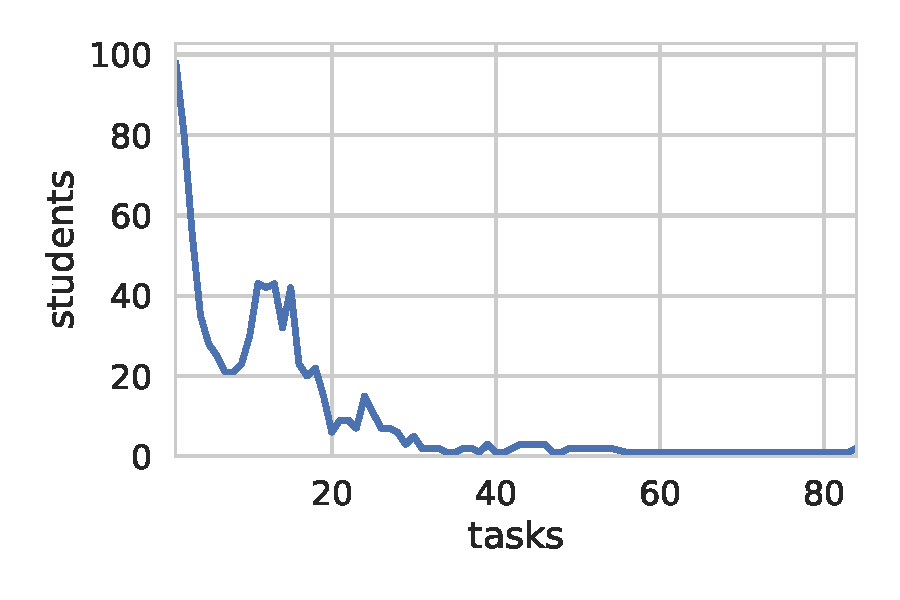
\includegraphics[height=42mm]{img/engagement-tasks}
%\caption{How many students solved given number of tasks.}
\end{subfigure}
\begin{subfigure}{.49\textwidth}
\centering
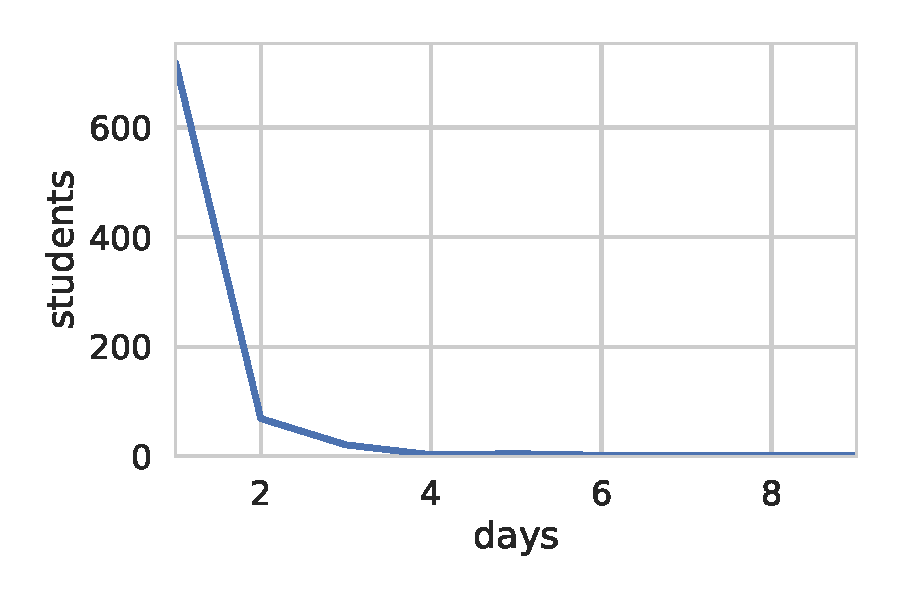
\includegraphics[height=42mm]{img/engagement-days}
%\caption{How many students solved a task given number of days.}
\end{subfigure}
\caption{%
  Engagement curves show how many students solved at least given number of tasks (left),
  and how many students solved a task at least given number of days (right).}
\label{fig:engagement-curves}
\end{figure}


About 11000 tasks were attempted (counting only attempts with at least one edit),
and 9600 of them were solved,
resulting in the overall success rate $86\%$.
The daily numbers of solved task sessions are not stable,
with high peaks on days when RoboMission was used
in a programming competition or Hour of Code session at a school
(\cref{fig:solved-count}).
% The following can be a separate paragraph, if another
% analysis is performed.
Over 180 thousand program snapshots was collected,
of which 140 thousand corresponds to edits
and 40 thousand to executions.

% TODO: join with another plot (-> two plots on a single line).
% (e.g., a metric mentioned at the theory part)
% TODO: crop/tighten margings (esp. the bottom one)
%\imgW[0.3]{daily-task-sessions}{%
%  Daily number of solved task sessions (weekly averaged).}
\begin{figure}[htb]
\centering
\begin{subfigure}{.49\textwidth}
\centering
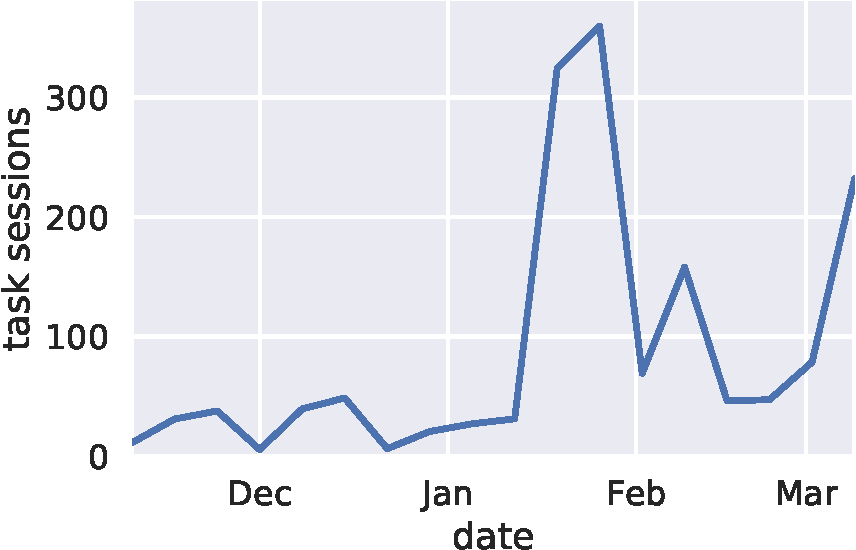
\includegraphics[height=39mm]{img/daily-task-sessions-cropped}
\caption{Daily number of solved tasks\\(weekly averaged).}
\label{fig:solved-count}
\end{subfigure}
\begin{subfigure}{.49\textwidth}
\centering
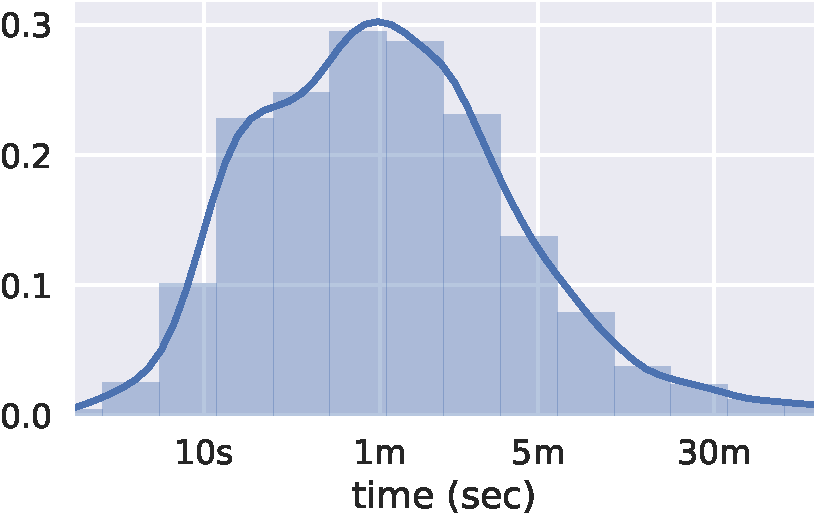
\includegraphics[height=39mm]{img/task-sessions-time-log-cropped}
\caption{Distribution of log-transformed solving times.}
\label{fig:solving-times-all}
\end{subfigure}
\caption{Task sessions.}
\label{fig:daily-task-sessions}
\end{figure}

Median solving time is 1 minute (interquartile range: 24--145 seconds).
Solving times follow log-normal distribution (\cref{fig:solving-times-all}),
so the mean solving time is much higher
(about 3 minutes). %195 seconds, % with high standard deviation of nearly 500 seconds.
% even if the times are capped at one hour).
% and not very informative


\section{System Behavior}

We can use the collected data to check the requirements on system behavior mentioned in
\cref{sec:robomission.behavior}. Unfortunately, the system is currently not logging
which tasks were recommended and which were self-selected, so we cannot determine
how much are the results influenced by the adaptive behavior. % of the system.
From all attempts, 86\% are successful, and 84\% are solved in less than 15 minutes.
If we look at the first 5 practiced tasks for each student, 87\% of them are solved,
85\% are solved in less than 15 minutes, but only 66\% are solved in less than 2 minutes.

% TODO: how to create horizontal space between them?
\begin{figure}[htb]
\centering
\begin{subfigure}{.48\textwidth}
\centering
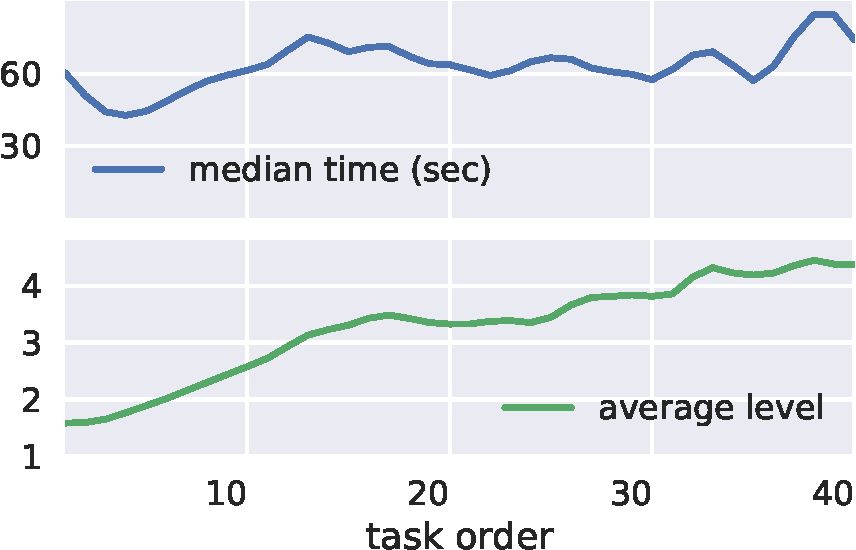
\includegraphics[height=40mm]{img/median-time-order-cropped}
\caption{Median solving time and average level per task order during practice.
  First 10 tasks have the median solving time below 1 minute.}
  % The median is below one minute for first 10 tasks.}
\label{fig:solving-times-per-order}
\end{subfigure}
\begin{subfigure}{.50\textwidth}
\centering
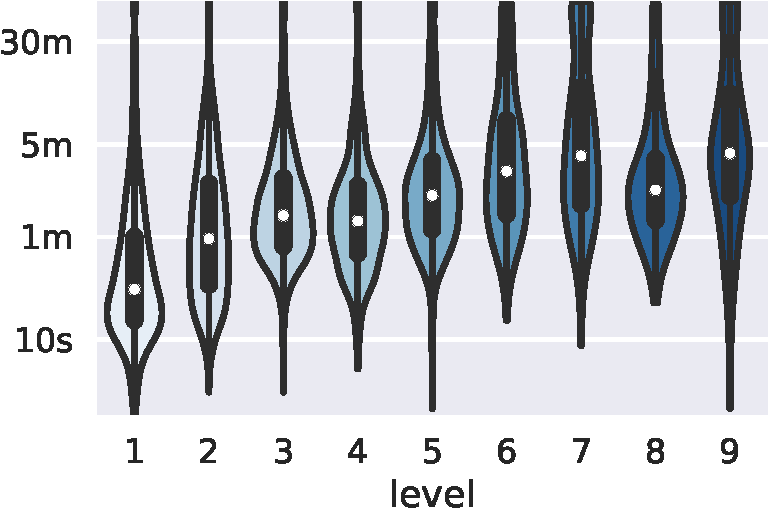
\includegraphics[height=40mm]{img/levels-time-cropped}
\caption{Distributions of log-transformed solving times for all levels,\\
         with highlighted medians and interquartile ranges.}
\label{fig:levels-time}
\end{subfigure}
\caption{Levels and solving times.}
\label{fig:solving-times}
\end{figure}


The median solving time of the first 10 practiced tasks is below 1 minute.
Surprisingly, the median time does not increase too much even for the later
attempts during practice (\cref{fig:solving-times-per-order}).
The curve of median times stays similar
if only students with at least 40 task sessions are used for the computation,
which rules out the possibility that this behavior is caused by \emph{attrition bias}
(only better students staying in the system, making the later tasks seem easier than they are).
The plot of the average level per task order during practice
(\cref{fig:solving-times-per-order} bottom) reveals a possible explanation:
an average student is still in the 4th level after 30 tasks,
and the 3rd and 4th level have similar difficulty with a median solving time below 90 seconds
(\cref{fig:levels-time}).
% + random recommendation of tasks from lower level + learning



After 10 minutes of practice, 73\% of students have reached the second level,
and after 20 minutes, nearly 70\% of students have started practicing loops.
Then the progress through levels slows down, and only 37\% of students
are practicing both loops and conditional statements after the first
hour of the tutorial (\cref{fig:students-at-levels}).

\begin{figure}[htb]
\centering
\begin{subfigure}{.49\textwidth}
\centering
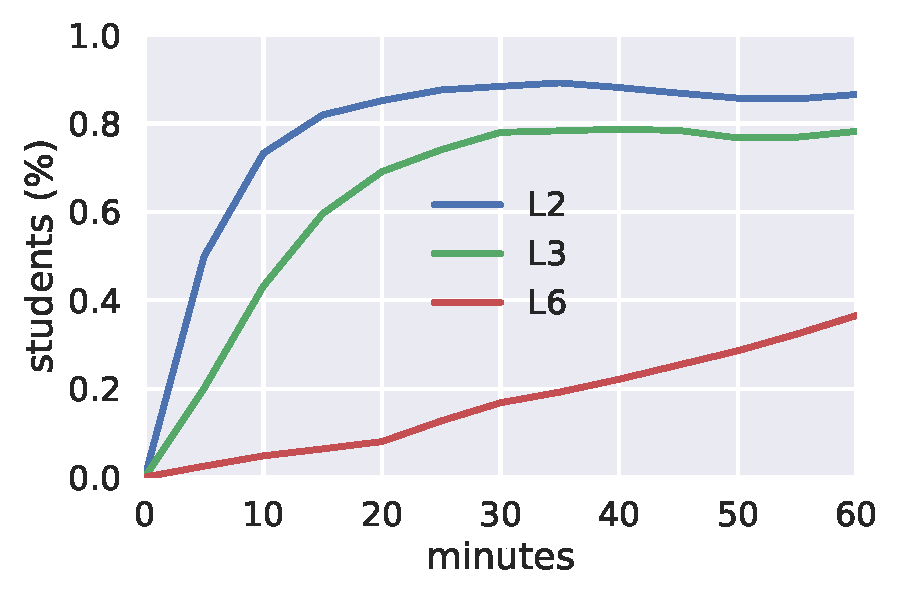
\includegraphics[height=42mm]{img/students-at-levels}
%\caption{How many students solved given number of tasks.}
\end{subfigure}
\begin{subfigure}{.49\textwidth}
\centering
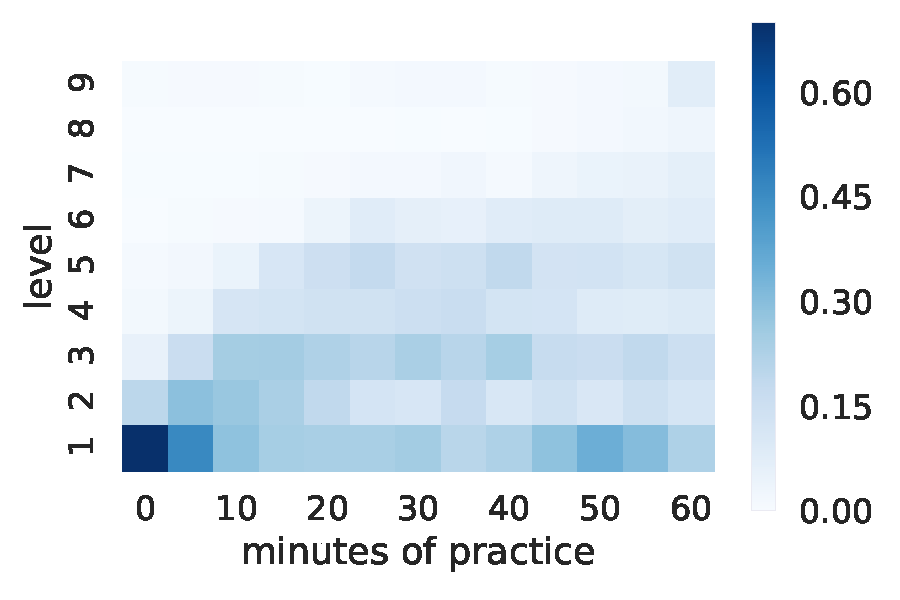
\includegraphics[height=42mm]{img/task-sessions-at-levels}
%\caption{How many students solved a task given number of days.}
\end{subfigure}
\caption{%
  Left: the proportion of students in the system after some time of practicing,
  who progressed to the 2nd, 3rd, and 6th level (sequence of commands, repeat loops, if-statements).
  Right: how the proportion of tasks at different levels is shifting during the practice.}
\label{fig:students-at-levels}
\end{figure}

\section{Performance Measurement}

% In ... we have discussed importance of a performance compression
Measurement of performance has an enormous impact on the estimated skills, %in the student model,
and transitively on %the behavior of the tutor model. %, e.g.,
the task recommendations. % to the student.
Currently, we measure %three-valued performance representation, and a
performance using only observed solving time
(\cref{sec:robomission.student}).
However, due to variations in speeds of different students
(which are influenced by external factors, such as used device),
solving time is a rather noisy approximation of the true performance.
Could using other observational data, such as the number of edits,
bring more information about the performance?

%(TODO: Goal: find a compression function that maximizes performance of student model.)
Overall Pearson correlation between solving times and the number of edits (both
log-transformed) is quite high, about 0.73 (\cref{fig:performance-corrs-ts}).
However, if computed for individual tasks,
median correlation drops to 0.64, % (interquartile range 0.5 -- 0.72),
and $25\%$ of tasks have correlation below 0.5 % check the number
(\cref{fig:time-vs-edits}), which suggests that incorporating the number of edits into the
measurement should be considered.

We propose the following heuristic for combining solving times with the number
of edits and runs (executions): a log-transformed sum of edits, runs, and \emph{thinking
actions}.
Thinking action is only assumed to be between two edits or runs if the time interval
is at least 5 seconds long, in order to reduce the noise caused, e.g., by
different screen sizes
(5 seconds seems to be enough to drag and drop a block anywhere on any screen).
If the interval is very long,
we count it as multiple thinking actions (taking $log_5$ from the time interval
and rounding it down to the closest integer).

With this definition, an average student performs about 5 thinking actions
in the first two levels (practicing only sequences of commands),
and about 10 thinking actions in the 3rd and 4th level (practicing repeat and while loops)
(\cref{fig:actions-thinkings}).
This heuristic retains reasonable correlation with both solving time
and number of edits for all tasks (\cref{fig:performance-corrs-p10}).

% the same with thresholds derived from task median (computing 3-level performance)
% -> measure agreement on all task sessions (not correlation, because specific
%  values are now important; prabably RMSE to penalize larger discrepances severaly).
% TODO: 3rd level of abstraction:
% - explore influence of different aggregations, e.g. all-mean (default), min-per-task, median-per-task,
% - explore the role of thresholds
% - explore influence of error metrics; of number of levels
% - explore usage in predictive models on the next performance (independent/cross)
% - explore the action-count measure (with thresholds): e.g., how it behaves wrt. incrasing levels


\begin{figure}[htb]
\centering
%\captionsetup[subfigure]{width=0.90\textwidth,justification=raggedright}%
\begin{subfigure}{.49\textwidth}
\centering
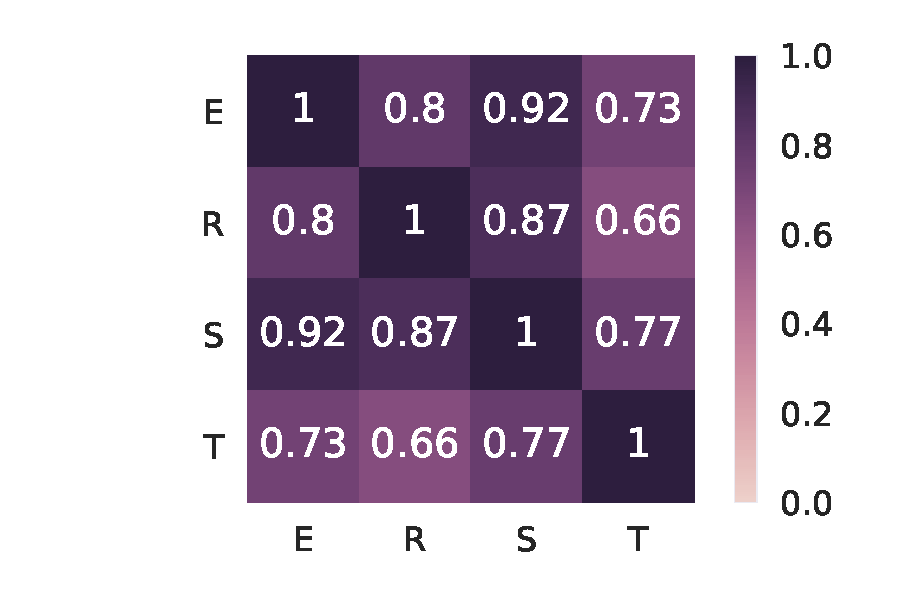
\includegraphics[height=49mm,trim={34mm 0 11mm 0},clip]{img/performance-corr-ts}
\caption{Pearson correlation between performance measures computed\\over all task sessions.}
\label{fig:performance-corrs-ts}
\end{subfigure}
%\begin{subfigure}{.33\textwidth}
%\centering
%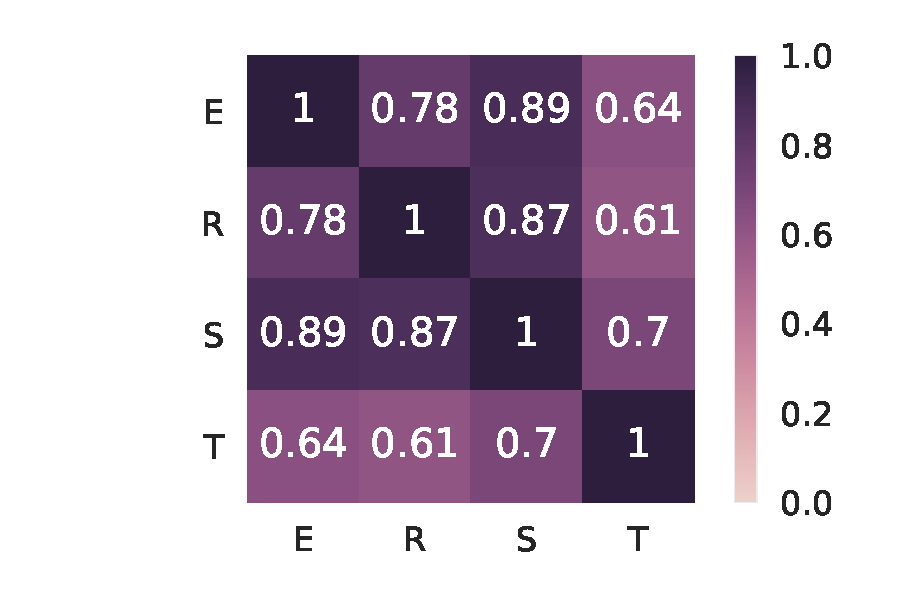
\includegraphics[height=32mm,trim={34mm 0 0 0},clip]{img/performance-corr-tasks-med}
%\caption{B.}
%\end{subfigure}
\begin{subfigure}{.49\textwidth}
\centering
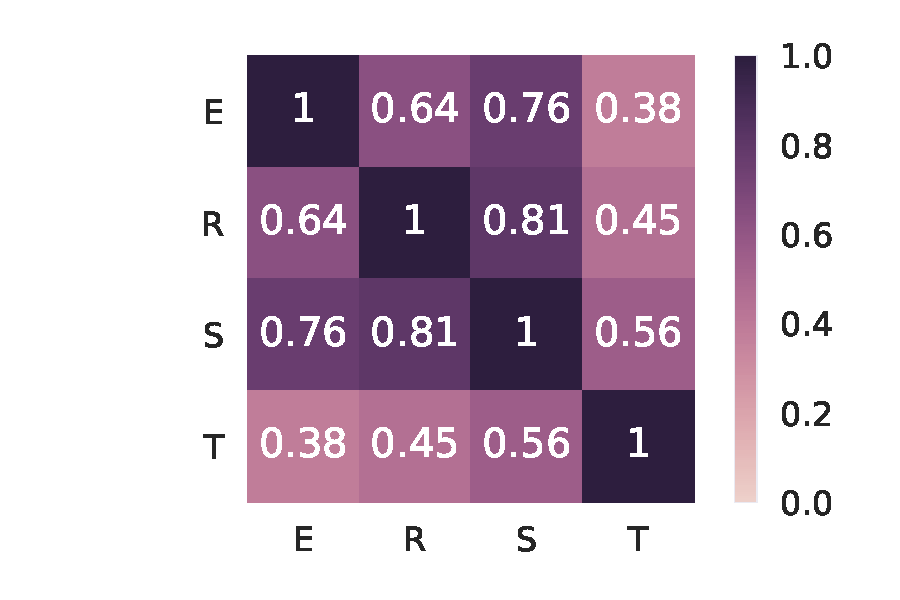
\includegraphics[height=49mm,trim={34mm 0 11mm 0},clip]{img/performance-corr-tasks-q10}
\caption{Aggregated per task, bottom 10th percentile
  (i.e., for 10\% of tasks the correlation is below the shown value).}
\label{fig:performance-corrs-p10}
\end{subfigure}
\caption{Correlation between four performance measures
(all of them log-transformed):
E = number of edits, R = number of runs, S = sum of edits, runs, and thinking actions,
T = solving time.}
\label{fig:performance-corrs}
\end{figure}


\begin{figure}[htb]
\centering
\begin{subfigure}{.49\textwidth}
\centering
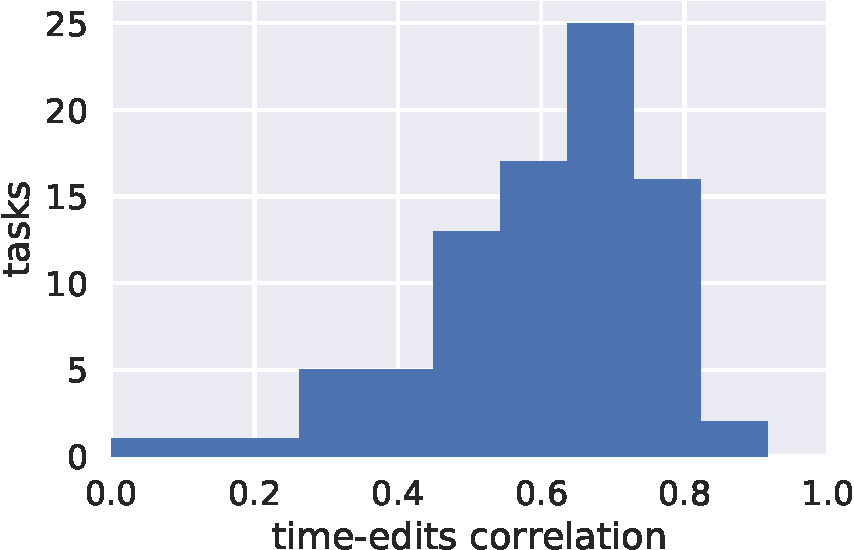
\includegraphics[height=38mm]{img/time-edits-corr-cropped}
\caption{
  Distribution of Pearson correlations between median solving times and number
  of edits (both log-transformed) for individual tasks.}
\label{fig:time-vs-edits}
\end{subfigure}
\begin{subfigure}{.49\textwidth}
\centering
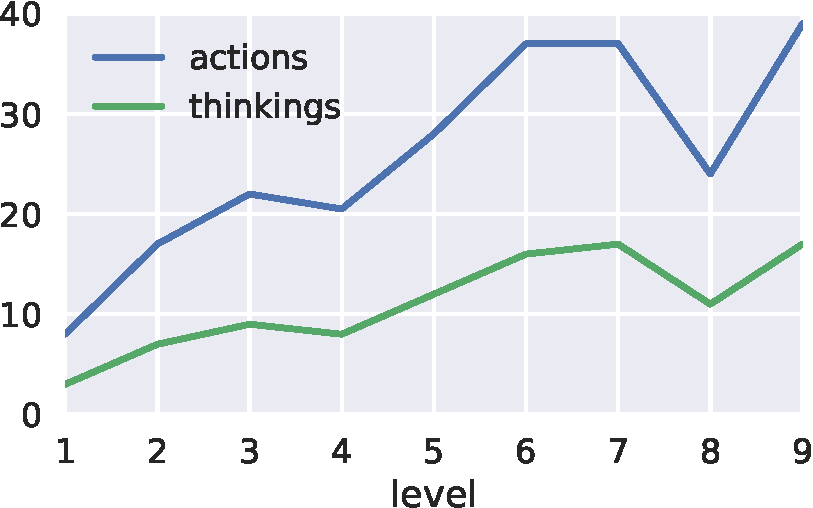
\includegraphics[height=39mm]{img/actions-thinkings-cropped}
\caption{Median number of actions (edits, runs, and thinking actions)
  with the increasing level.\\~}
\label{fig:actions-thinkings}
% TODO: add interquartile ranges
\end{subfigure}
\caption{Analysis of performance measures.}
\end{figure}


\begin{figure}[htb]
\centering
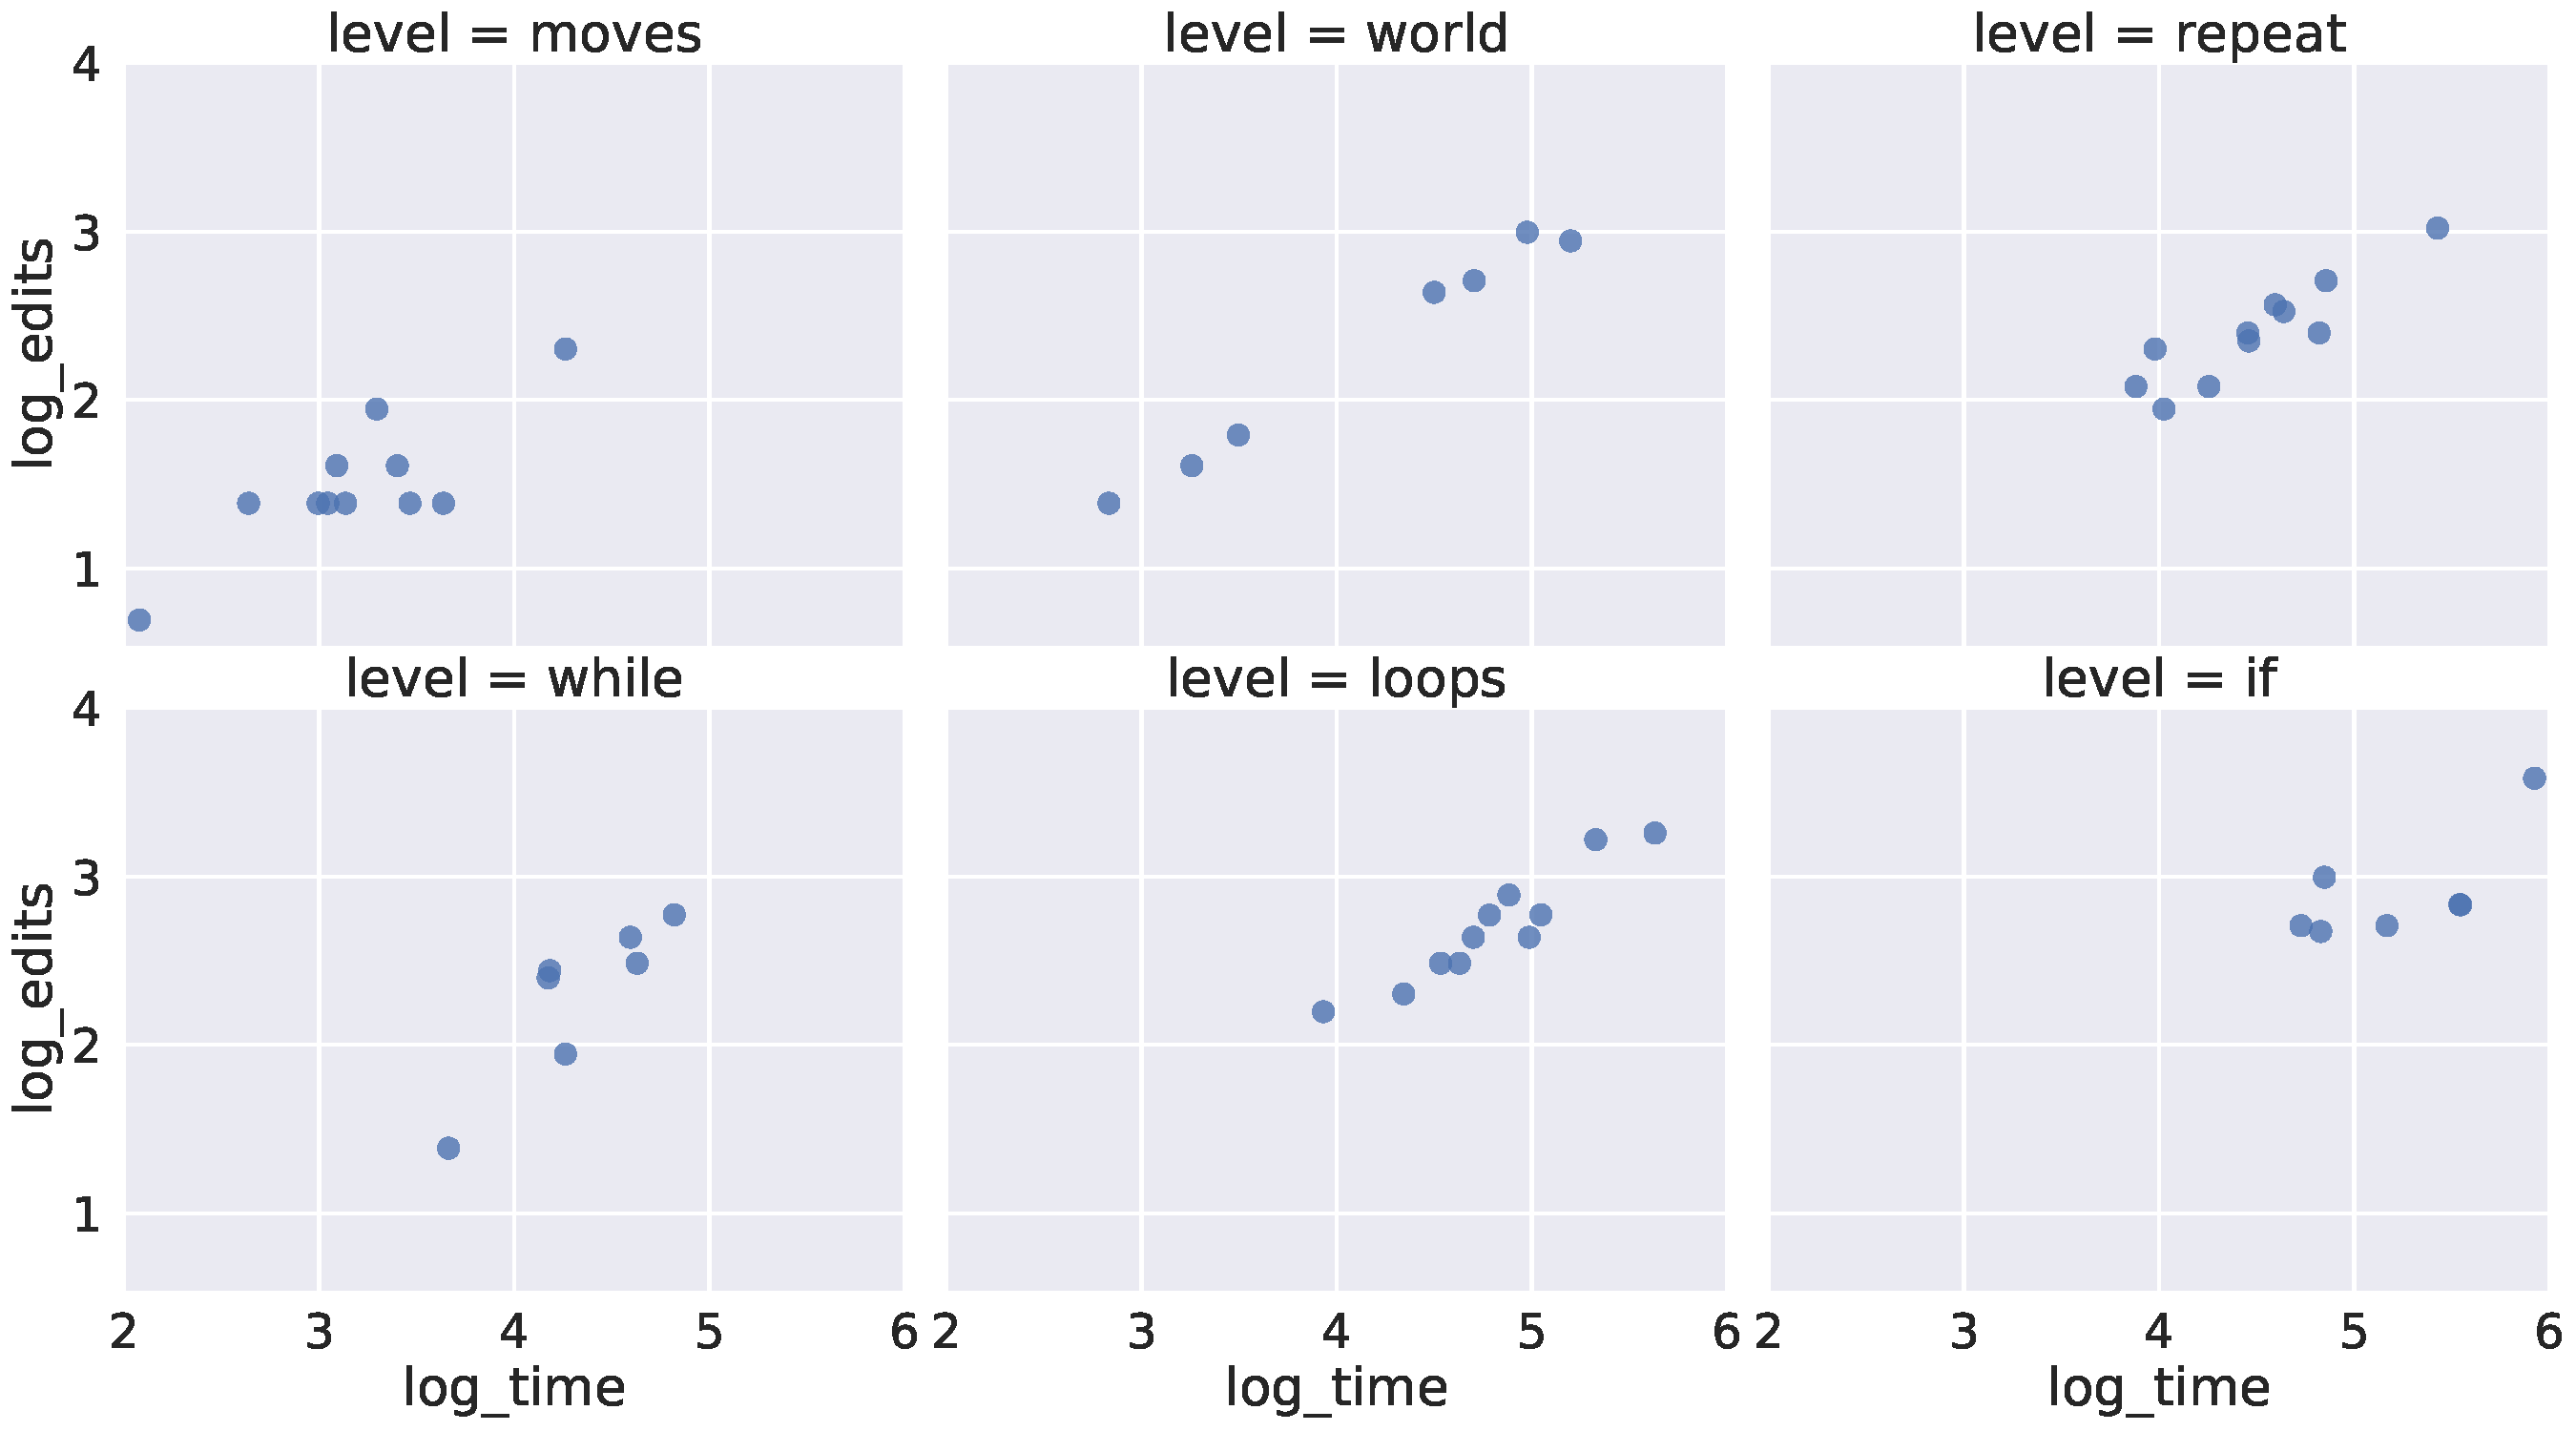
\includegraphics[width=\textwidth]{img/difficulties-tasks-levels}
\caption{%
  Difficulties of tasks in the first 6 levels.
  The difficulty is measured as success rate and median solving time.}
\label{fig:difficulties-tasks-levels}
\end{figure}




\section{Task Difficulties}

% Reformulate to make it clear, that it is the analysis before introduction of the phases,
% that actually leads to the refinement described in the thesis.

% TODO: Resolve mission vs. level.
Our tutor model (\cref{robomission.tutor}) assumes that difficulties of tasks
in each phase are approximately the same,
and that the overall difficulty is increasing as the level increases.   % even phase.
Using collected data, we can determine whether these assumptions are satisfied,
and if not, suggest adjustments to improve their validity.
\Cref{fig:levels-time} shows that on average the difficulty of levels
is increasing, but it also reveals that level 7 is more difficult than level 8.
Levels 3 and 4 have similar difficulty, which is expected because they practice
two similar concepts, repeat and while loops.

% TODO: Elaborate on the solution to this issue.
% (TODO?: phases instead of missions, and select only a few to save space)
Looking at the difficulty of individual tasks (\cref{fig:difficulties-tasks-levels})
help us to discover outliers, whose difficulty is significantly
different from the other tasks in the same level.
The \cref{fig:difficulties-tasks-levels} also suggests that dividing levels
into phases is necessary to achieve reasonable homogeneity. For example, in the 2nd
level (World), there are two clear groups of tasks with significantly different
difficulty. Although in the other levels such a clear split does not exist,
they still contain tasks with a wide range of difficulties. %, so the refinement into phases seems appropriate.
% TODO: note/analyze robustness of these analyses (given the limited data)

%\imgW{difficulties-tasks-levels}{%
%  Difficulties (spent times and number of edits, both log-transformed)
%  of tasks in each level.}
